\documentclass[../Carre_nights.tex]{subfiles}

\begin{document}

\section{n0488}
\textbf{\Large{The tale of Abu Kir and Abu Sir}} \\

\begin{figure}[ht]
\centering
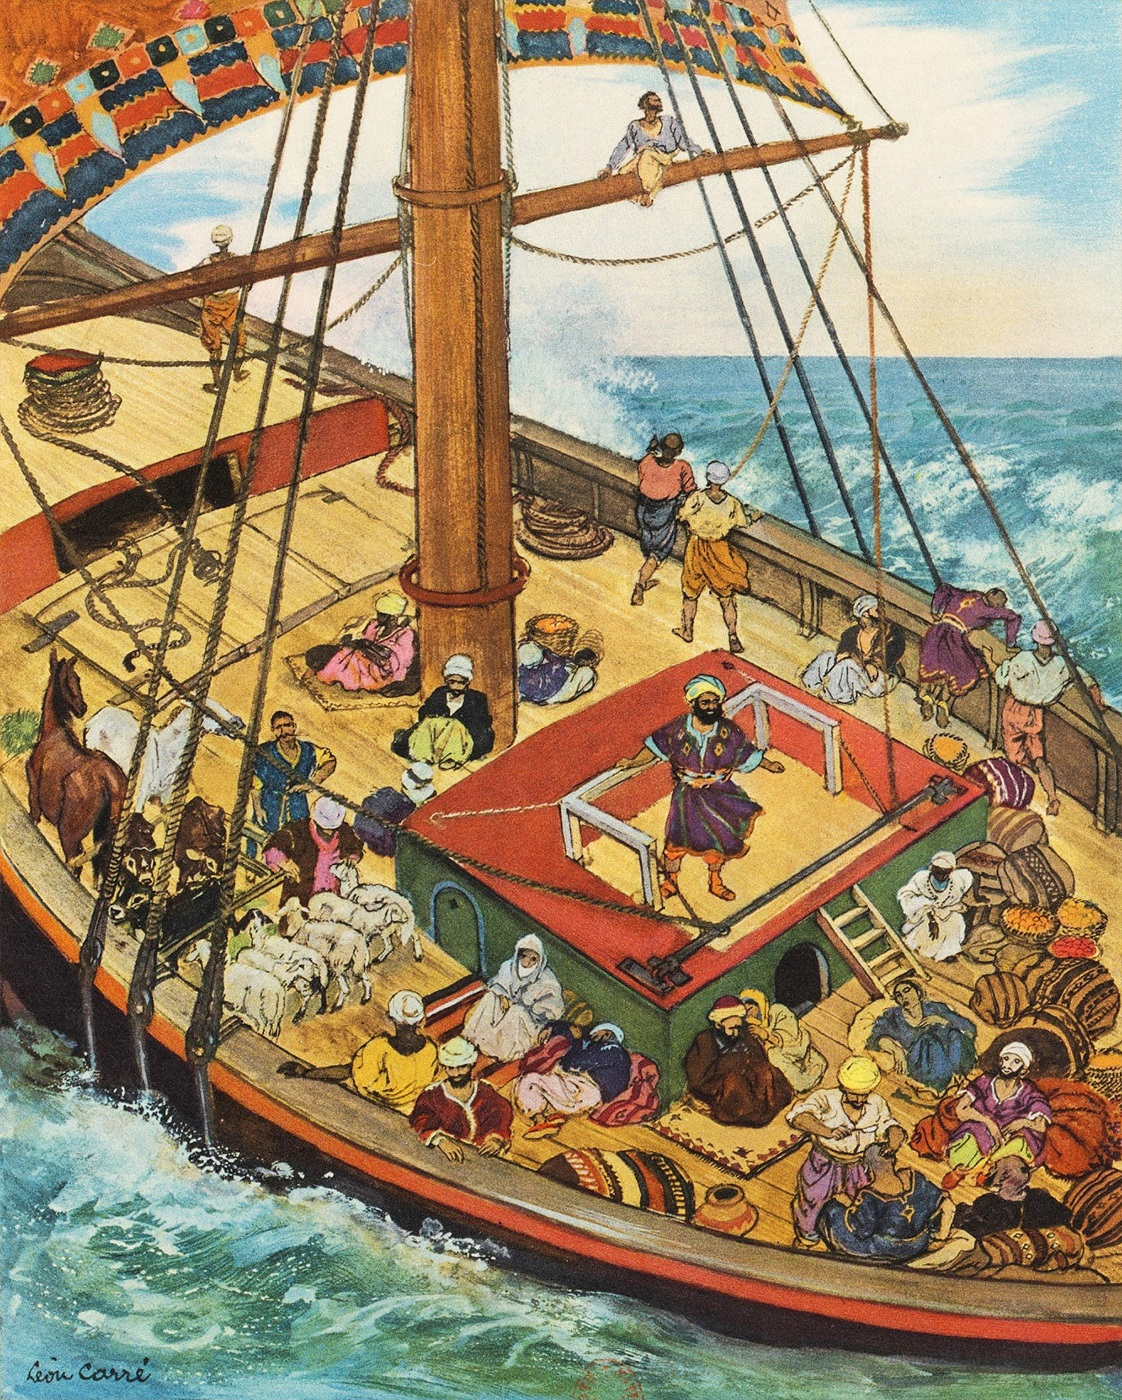
\includegraphics[height=\figsize]{illustrations/volume_5/T05, n0488 - Histoire d'Abou-Kir et d'Abou-Sir.jpg}
\end{figure}

\textit{\\
"...parmi les passagers et l’équipage dont le nombre s’élevait en tout à cent quarante hommes, sans compter le capitaine, il n’y avait point d’autre barbier qu’Abou-Sir..."} \\
—T05, n0488 - Histoire d'Abou-Kir et d'Abou-Sir \\~\\
\textit{"Among the passengers and crew, who numbered a hundred and forty souls, there was no other barber than Abu Sir..."} \\
—V03, n0488 - The tale of Abu Kir and Abu Sir

\newpage

\section{n0494}
\textbf{\Large{The tale of Abu Kir and Abu Sir}} \\

\begin{figure}[ht]
\centering
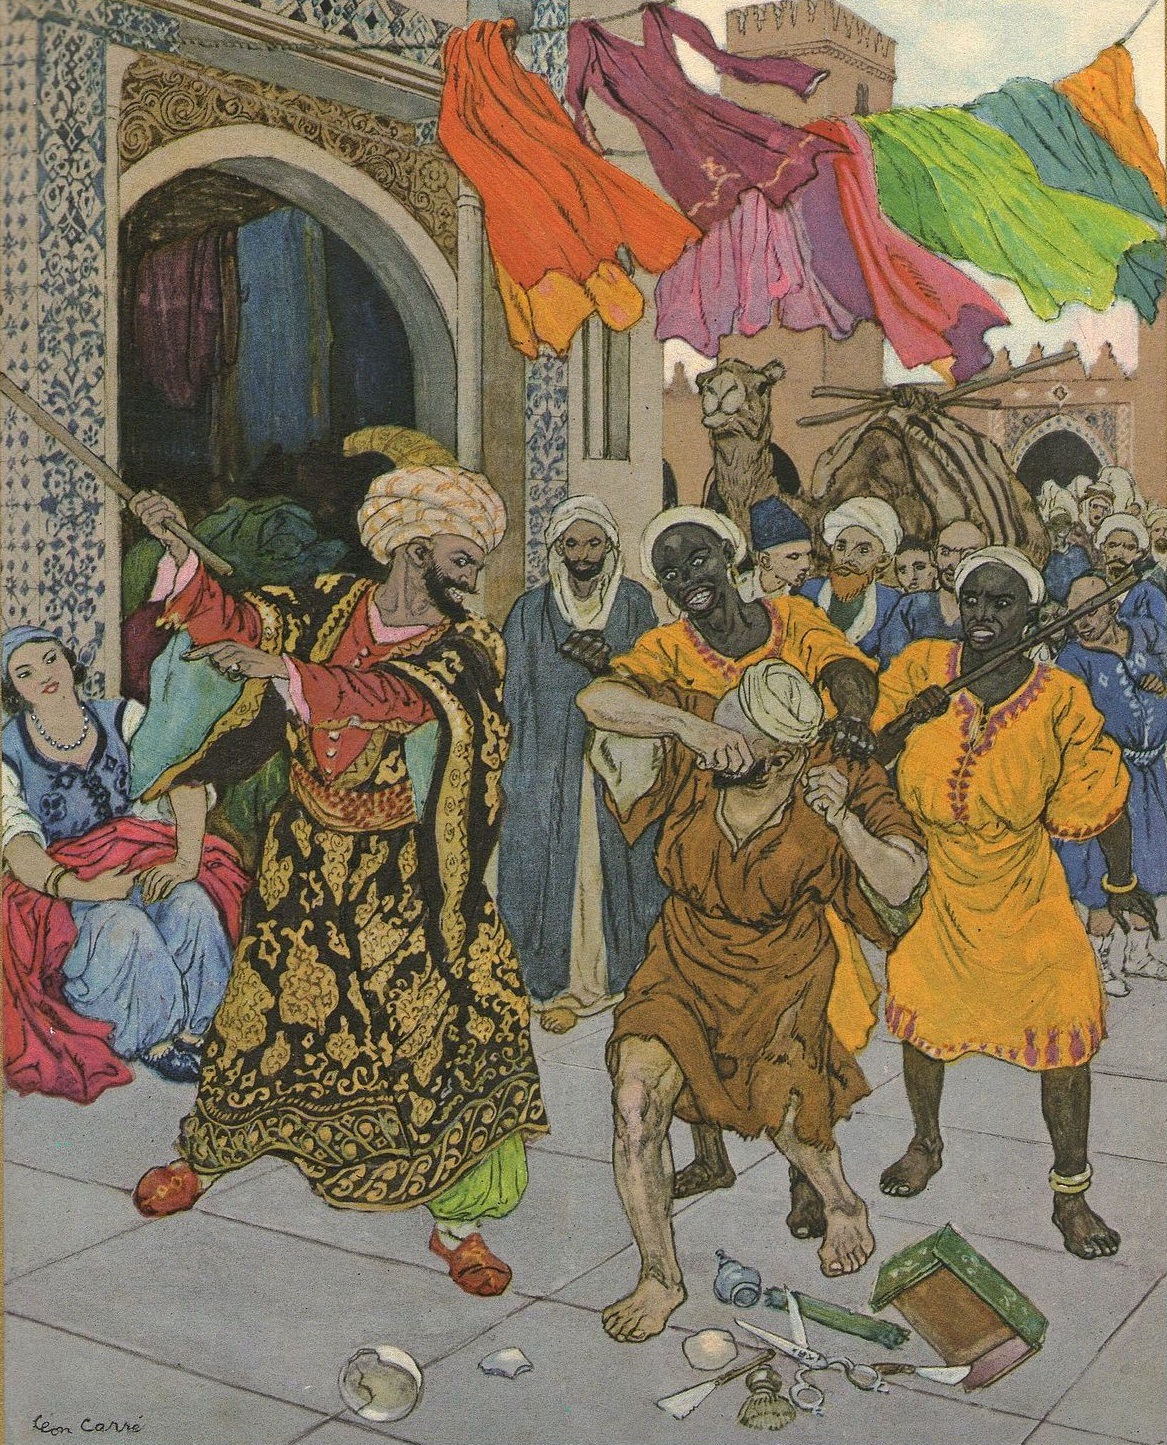
\includegraphics[height=\figsize]{illustrations/volume_5/T05, n0494 - Histoire d'Abou-Kir et d'Abou-Sir.jpg}
\end{figure}

\textit{\\
"...les esclaves blancs et les noirs se précipitèrent sur le pauvre barbier, et le renversèrent et le piétinèrent ; et le teinturier lui-même se leva, prit un grand bâton et dit : « Étendez-le sur le ventre ! »"} \\
—T05, n0494 - Histoire d'Abou-Kir et d'Abou-Sir \\~\\
\textit{"The white and black slaves leapt upon the unfortunate barber, threw him to the ground and trampled upon him; the dyer rose and took up a great stick, saying: 'Stretch him on his belly!'"} \\
—V03, n0494 - The tale of Abu Kir and Abu Sir

\newpage

\section{n0506}
\textbf{\Large{The tale of land Abdallah and sea Abdallah}} \\

\begin{figure}[ht]
\centering
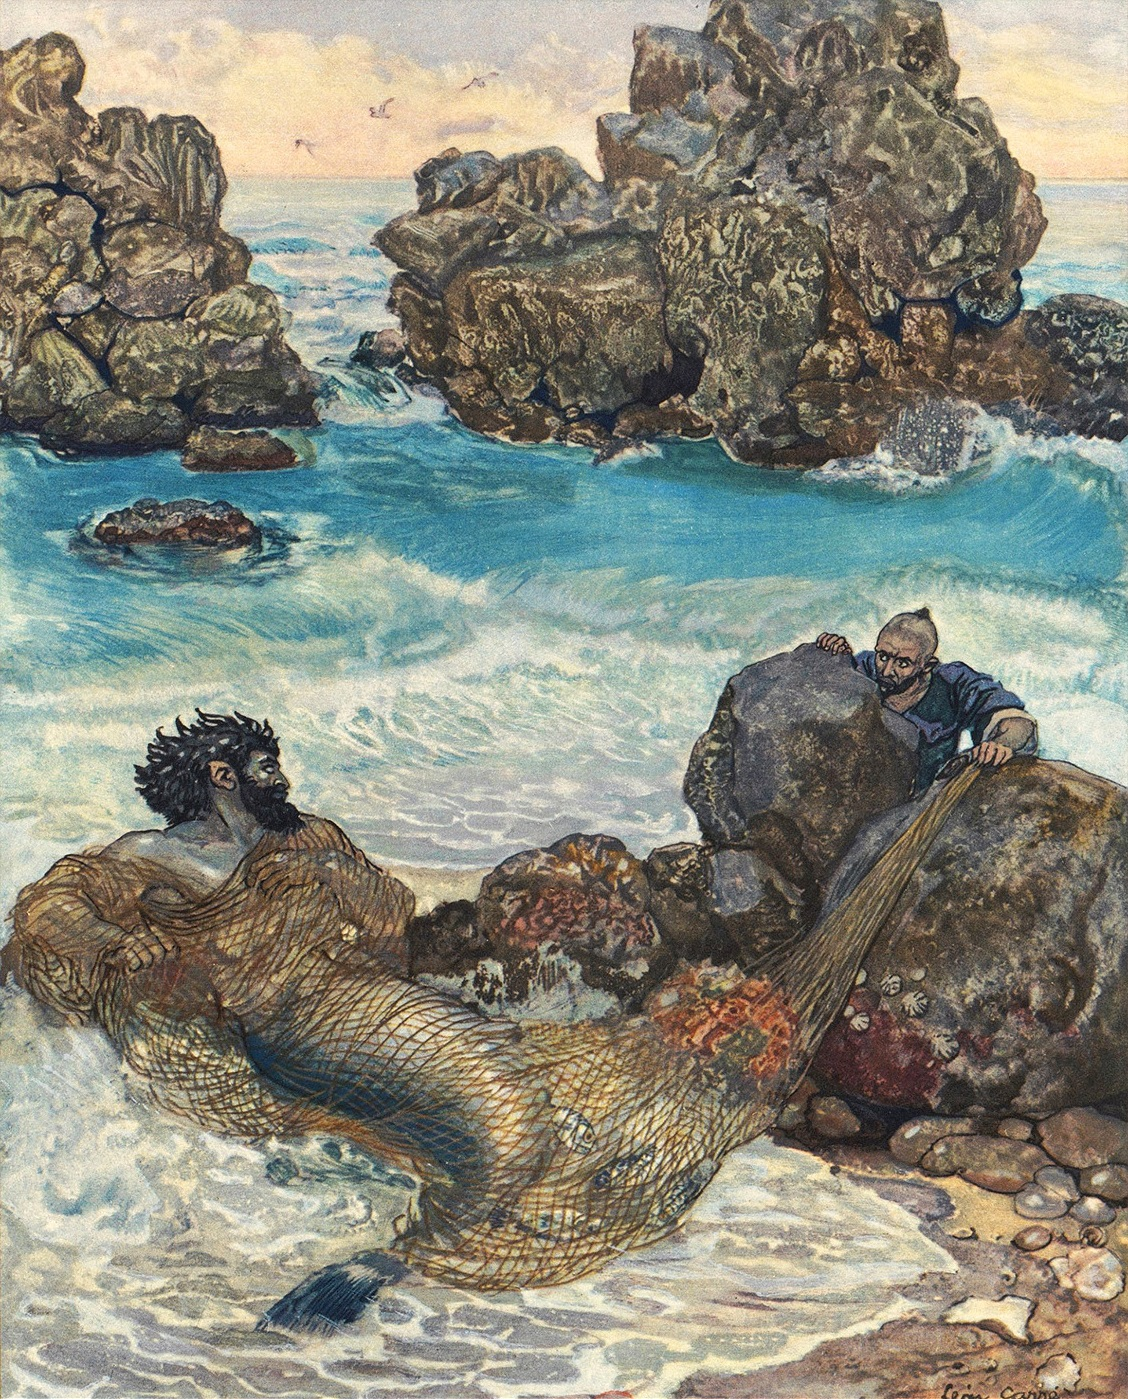
\includegraphics[height=\figsize]{illustrations/volume_5/T05, n0506 - Histoire d'Abdallah de la terre et d'Abdallah de la mer.jpg}
\end{figure}

\textit{\\
"...à la limite de la stupéfaction, il trouva, engagé entre les mailles du filet, un être humain, un Adamite, semblable à tous les Ibn-Adam, avec cette seule différence que son corps se terminait en queue de poisson, mais, à part cela, il avait une tête, un visage, une barbe, un tronc et des bras, tout comme un homme de la terre."} \\
—T05, n0506 - Histoire d'Abdallah de la terre et d'Abdallah de la mer \\~\\
\textit{"...to his stupefaction, he saw a human being, a son of Adam, caught in the meshes of the net. The apparition had a head, face, beard, trunk, and arms like ordinary men, but ended in a fish's tail."} \\
—V03, n0506 - The tale of land Abdallah and sea Abdallah

\newpage

\section{n0513}
\textbf{\Large{The tale of land Abdallah and sea Abdallah}} \\

\begin{figure}[ht]
\centering
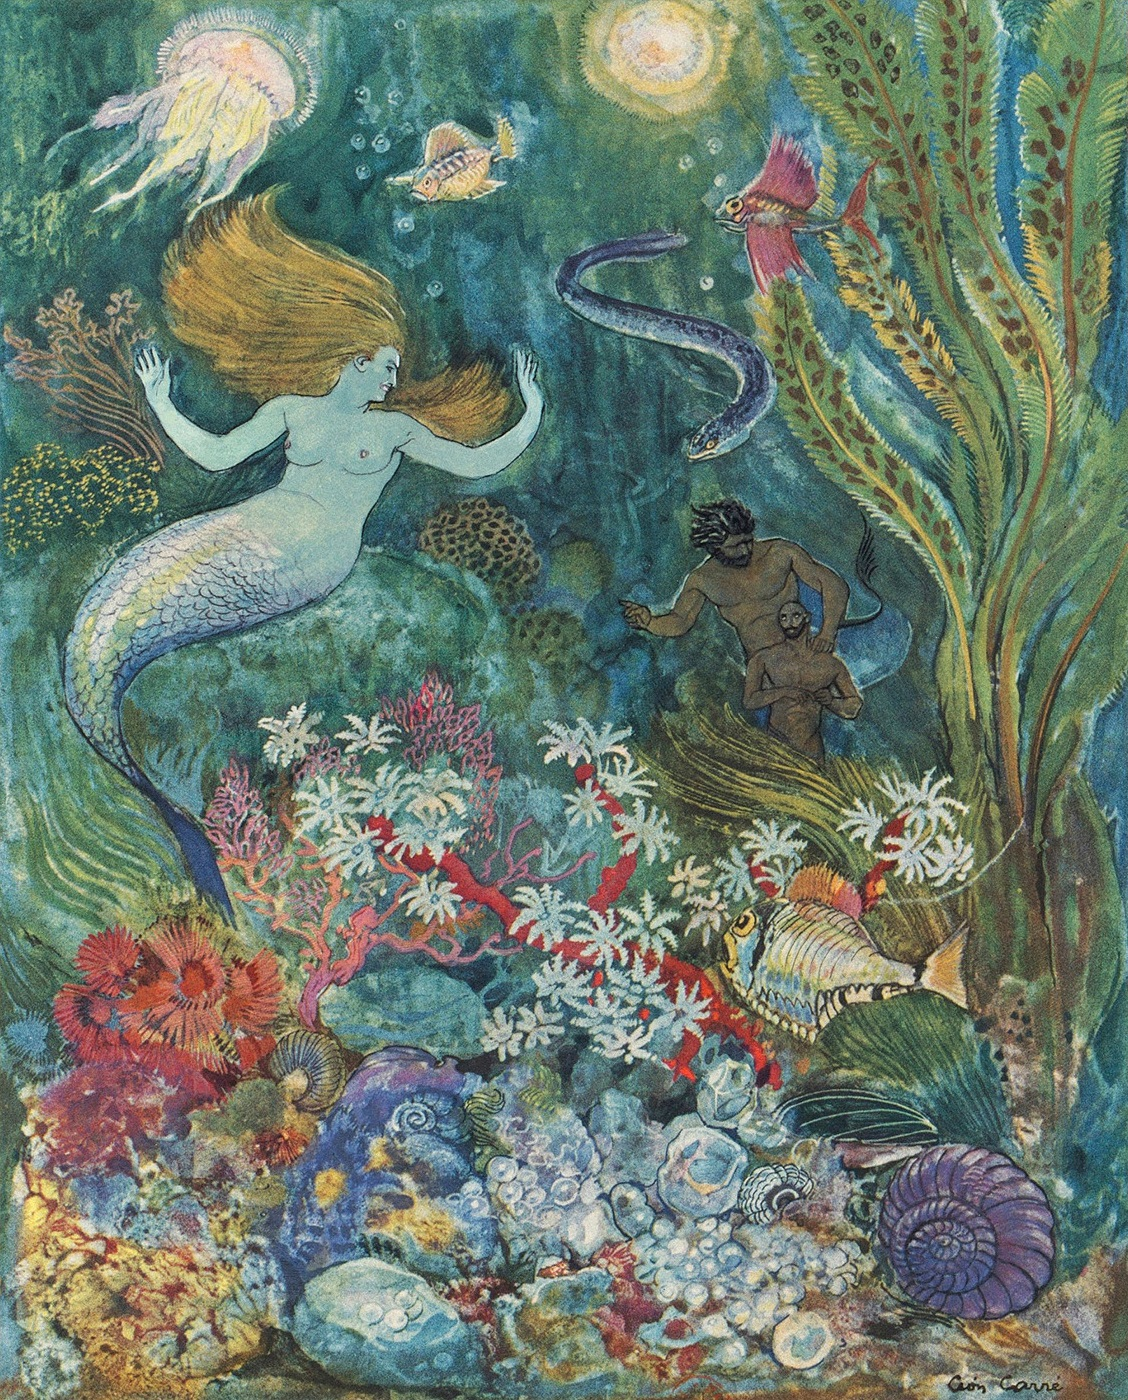
\includegraphics[height=\figsize]{illustrations/volume_5/T05, n0513 - Histoire d'Abdallah de la terre et d'Abdallah de la mer.jpg}
\end{figure}

\textit{\\
"...soudain Abdallah le Terrien, qui, toujours au bras de son ami, voyait défiler devant lui, en une course rapide sur les abîmes, tous ces spectacles splendides, aperçut une innombrable suite de cavernes d’émeraude, taillées à même les flancs d’une montagne de la même gemme verte, et aux portes desquelles étaient assises ou étendues des adolescentes belles comme des lunes, aux cheveux couleur de l’ambre et du corail."} \\
—T05, n0513 - Histoire d'Abdallah de la terre et d'Abdallah de la mer \\~\\
\textit{"Suddenly Land Abdallah who, walking always with his arm in his friend's, watched these strange beauties defile past him, saw a long terrace of caves, cut in the flanks of a mountain of emerald. At the doors sat or stood girls, silvered like the moon, with amber coloured hair."} \\
—V03, n0513 - The tale of land Abdallah and sea Abdallah

\newpage

\section{n0516}
\textbf{\Large{The tale of the yellow youth}} \\

\begin{figure}[ht]
\centering
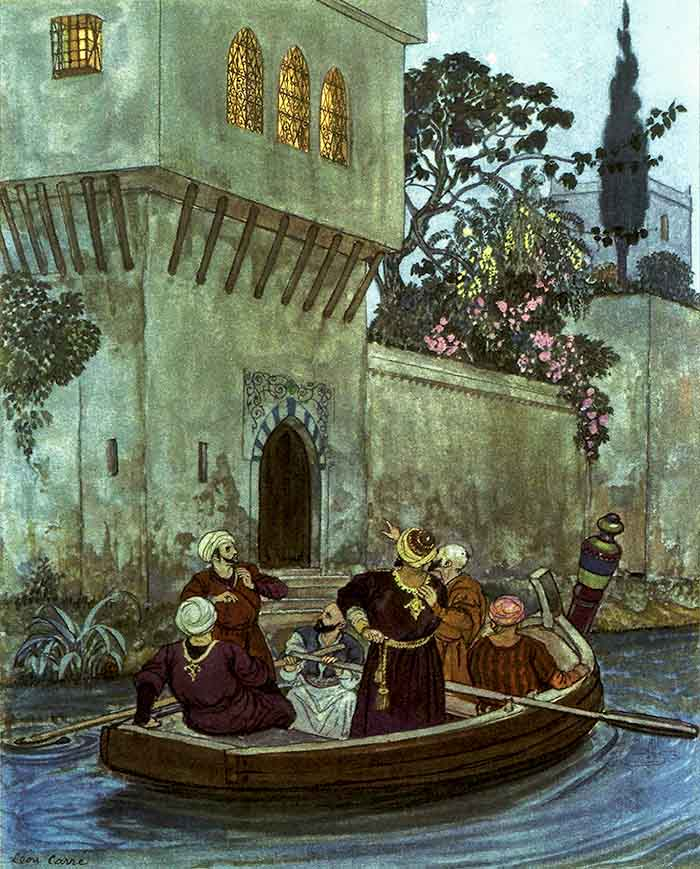
\includegraphics[height=\figsize]{illustrations/volume_5/T05, n0516 - Histoire du jeune homme jaune.jpg}
\end{figure}

\textit{\\
"...le khalifat dit : « Pénétrons, ô Giafar, dans cette maison pour demander l’hospitalité au maître du lieu, dans l’espoir de mieux entendre cette voix ! »"} \\
—T05, n0516 - Histoire du jeune homme jaune \\~\\
\textit{"Then said the Khalifah: 'Let us ask hospitality from the master of this house, and perhaps, in that way, we may get to hear the voice more clearly.'"} \\
—V03, n0516 - The tale of the yellow youth

\newpage

\section{n0527}
\textbf{\Large{The tale of Pomegranate-Flower and Badr Basim}} \\

\begin{figure}[ht]
\centering
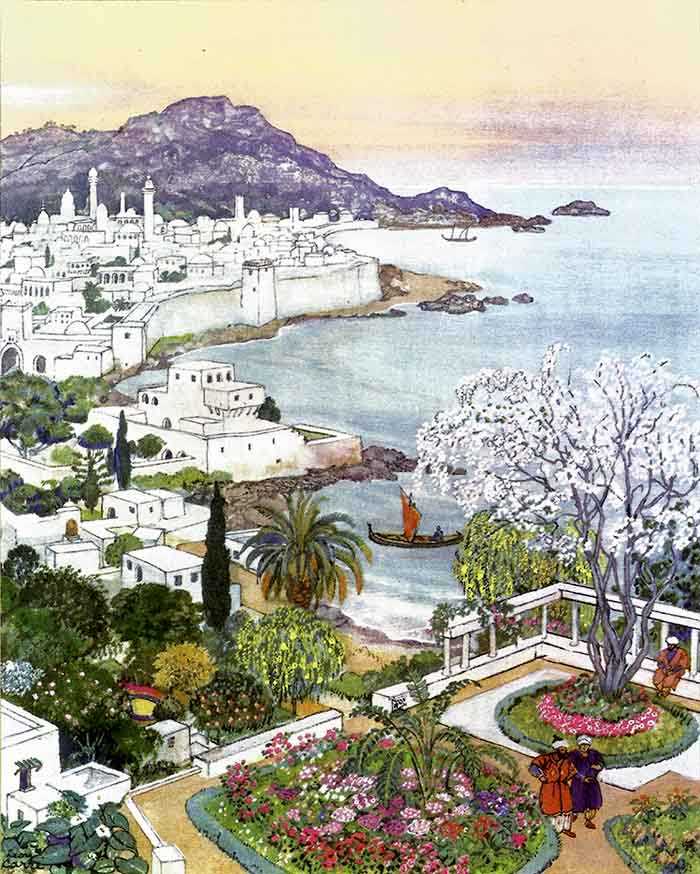
\includegraphics[height=\figsize]{illustrations/volume_5/T05, n0527 - Histoire de Fleur-de-Grenade et de Sourire-de-Lune.jpg}
\end{figure}

\textit{\\
"...la ville capitale où régnait le roi Schahramân se trouvait en effet, située sur le bord de la mer, et son nom était la Ville-Blanche. Et c’est ainsi que les femmes du palais purent conduire, après le bain, l’adolescente étrangère dans un pavillon qui regardait la mer."} \\
—T05, n0527 - Histoire de Fleur-de-Grenade et de Sourire-de-Lune \\~\\
\textit{"...the capital of King Shahriman, which was called the White Town, stood on the sea shore; and it was thus possible for the women of the palace to give the stranger a pavilion overlooking the waters."} \\
—V03, n0527 - The tale of Pomegranate-Flower and Badr Basim

\newpage

\section{n0541}
\textbf{\Large{The tale of Pomegranate-Flower and Badr Basim}} \\

\begin{figure}[ht]
\centering
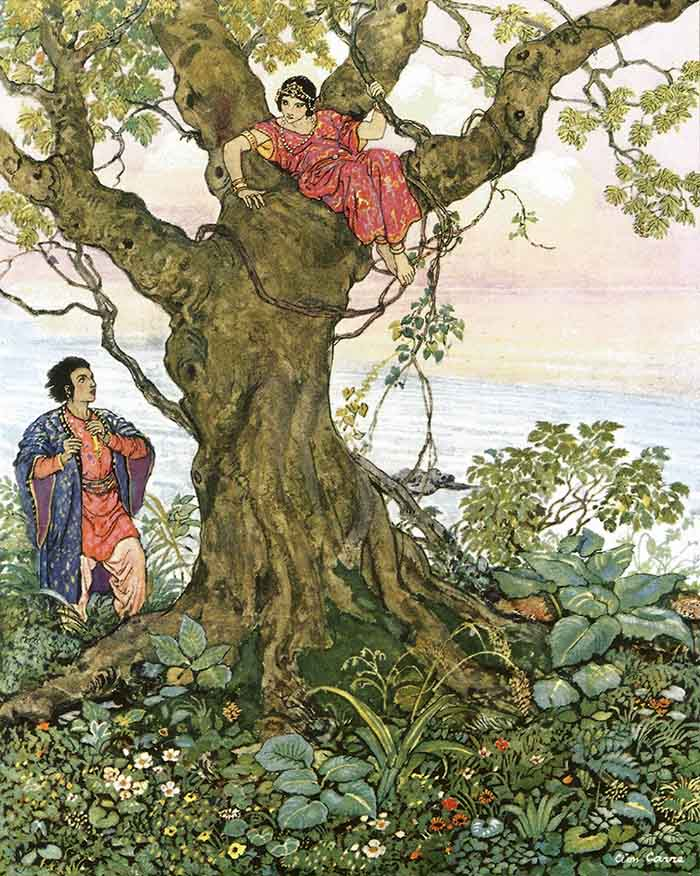
\includegraphics[height=\figsize]{illustrations/volume_5/T05, n0541 - Histoire de Fleur-de-Grenade et de Sourire-de-Lune.jpg}
\end{figure}

\textit{\\
"...ému à l’extrême, il sauta sur ses pieds et, se tenant debout au-dessous de l’arbre, il leva les yeux vers l’adolescente et lui dit : « Ô but suprême de tout désir, qui es-tu et pour quel motif te trouves-tu dans cette île, au haut de cet arbre ? »"} \\
—T05, n0541 - Histoire de Fleur-de-Grenade et de Sourire-de-Lune \\~\\
\textit{"He leapt to his feet in great emotion and, standing below the tree, lifted his eyes to the girl and said: 'O supreme goal of all desire, who are you and why are you mounted on a tree in this island?'"} \\
—V03, n0541 - The tale of Pomegranate-Flower and Badr Basim

\newpage

\section{n0555}
\textbf{\Large{The tale of Khalifah the fisherman}} \\

\begin{figure}[ht]
\centering
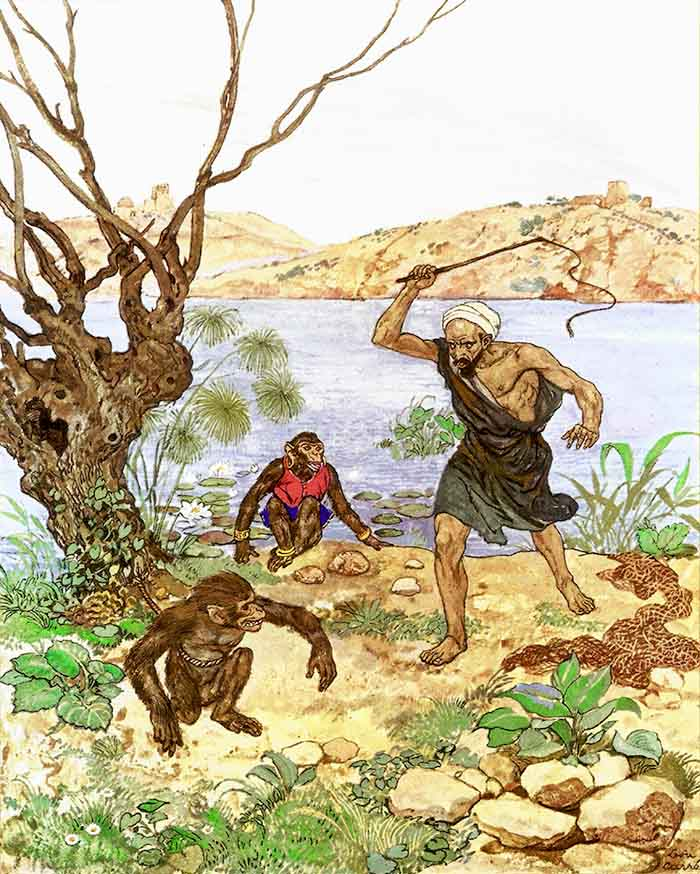
\includegraphics[height=\figsize]{illustrations/volume_5/T05, n0555 - Histoire de Khalife et du khalifat.jpg}
\end{figure}

\textit{\\
"...il courut vers le singe borgne attaché à l’arbre, et leva sur lui son fouet qu’il fit tournoyer d’abord trois fois dans l’air, en criant : « Regarde, ô visage de mauvais augure, ce qui résulte pour moi du conseil que tu m’as donné !"} \\
—T05, n0555 - Histoire de Khalife et du khalifat \\~\\
\textit{"...he ran towards the tree and, cracking his whip three times in the air, cried to his first captive: 'Look, O face of calamity, upon the result of your counsels!"} \\
—V03, n0555 - The tale of Khalifah the fisherman

\newpage

\section{n0571}
\textbf{\Large{The tale of Khalifah the fisherman}} \\

\begin{figure}[ht]
\centering
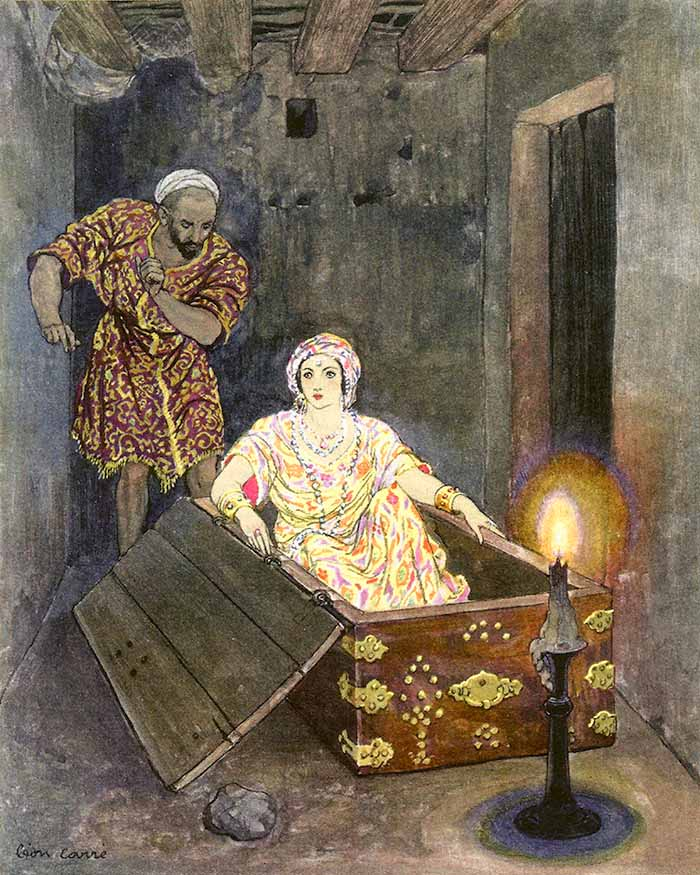
\includegraphics[height=\figsize]{illustrations/volume_5/T05, n0571 - Histoire de Khalife et du khalifat.jpg}
\end{figure}

\textit{\\
"...il prit une grosse pierre et brisa la serrure du coffre, et fit sauter du coup le couvercle ! Et il vit, étendue au-dedans, languissante et les pau- pières entrouvertes, une adolescente belle comme une houri, et brillante de pierreries."} \\
—T05, n0571 - Histoire de Khalife et du khalifat \\~\\
\textit{"He took up a large stone and, summoning all his courage, broke the lock of the chest and pulled back the lid. Inside he saw a girl as beautiful as the huris and all shining in the little light with diamonds."} \\
—V03, n0571 - The tale of Khalifah the fisherman

\newpage

\section{n0580}
\textbf{\Large{The adventures of Hasan of Basrah}} \\

\begin{figure}[ht]
\centering
\includegraphics[height=\figsize]{illustrations/volume_5/T05, n0580 - Les aventures de Hassân Al-Bassri.jpg}
\end{figure}

\textit{\\
"Commence donc par allumer ton fourneau, mets ton creuset sur le feu et fais marcher tes soufflets ! Puis, prends ce vieux plateau de cuivre et coupe-le en petites pièces avec les ciseaux !"} \\
—T05, n0580 - Les aventures de Hassân Al-Bassri \\~\\
\textit{"Light your furnace, put the crucible on the fire, and use your bellows. Then cut up the old dish with your scissors."} \\
—V03, n0580 - The adventures of Hasan of Basrah

\newpage

\section{n0596(1)}
\textbf{\Large{The adventures of Hasan of Basrah}} \\

\begin{figure}[ht]
\centering
\includegraphics[height=\figsize]{illustrations/volume_5/T05, n0596(1) - Les aventures de Hassân Al-Bassri.jpg}
\end{figure}

\textit{\\
"...Massrour les conduisit de la sorte dans le palais du khalifat, jusque devant le large trône bas où était majestueusement assise, au repos, El-Saiéda Zobéida, entourée de la foule nombreuse de ses esclaves femmes et de ses favorites..."} \\
—T05, n0596(1) - Les aventures de Hassân Al-Bassri \\~\\
\textit{"On arriving at the Khalifah's palace, the two women were led into the presence of Zubaidah, who sat at ease upon a broad low throne, surrounded by her women and her favourites."} \\
—V03, n0596(1) - The adventures of Hasan of Basrah

\newpage

\section{n0596(2)}
\textbf{\Large{The adventures of Hasan of Basrah}} \\

\begin{figure}[ht]
\centering
\includegraphics[height=\figsize]{illustrations/volume_5/T05, n0596(2) - Les aventures de Hassân Al-Bassri.jpg}
\end{figure}

\textit{\\
"...elle fit signe à Tohfa qui s’approcha aussitôt, en rougissant, de Splendeur, et commença par toucher le pan de son voile, pour porter ensuite à ses lèvres et à son front ses doigts qui avaient frôlé l’étoffe. Puis elle l’aida à rejeter son grand voile, et lui releva elle-même son petit voile de visage."} \\
—T05, n0596(2) - Les aventures de Hassân Al-Bassri \\~\\
\textit{"...she signed to Tuhfah, who went up to the stranger with a blush and began by touching the fringe of her garment. She carried the fingers which had touched it to her lips and brow, before helping Splendour to throw aside her great veil and lift the little gauze from before her face."} \\
—V03, n0596(2) - The adventures of Hasan of Basrah

\newpage

\section{n0607}
\textbf{\Large{The adventures of Hasan of Basrah}} \\

\begin{figure}[ht]
\centering
\includegraphics[height=\figsize]{illustrations/volume_5/T05, n0607 - Les aventures de Hassân Al-Bassri.jpg}
\end{figure}

\textit{\\
"...blanches et légères, elles descendirent dans la mer. Et l’écume se mêla à leurs chevelures libres et roulées, ou coiffées et hautes comme des tours. Et le gonflement des vagues continua le gonflement de leurs croupes vierges. Et elles étaient comme des corolles effeuillées sur les eaux."} \\
—T05, n0607 - Les aventures de Hassân Al-Bassri \\~\\
\textit{"...white and lightly they went down into the sea. The foam fell like flower petals upon their hair, free and wantoning, or built high in towers above their brow; the swelling waves imitated the curves of them; they were like sea-flowers budding above the water."} \\
—V03, n0607 - The adventures of Hasan of Basrah

\newpage

\section{n0622}
\textbf{\Large{The tale of the sleeper wakened}} \\

\begin{figure}[ht]
\centering
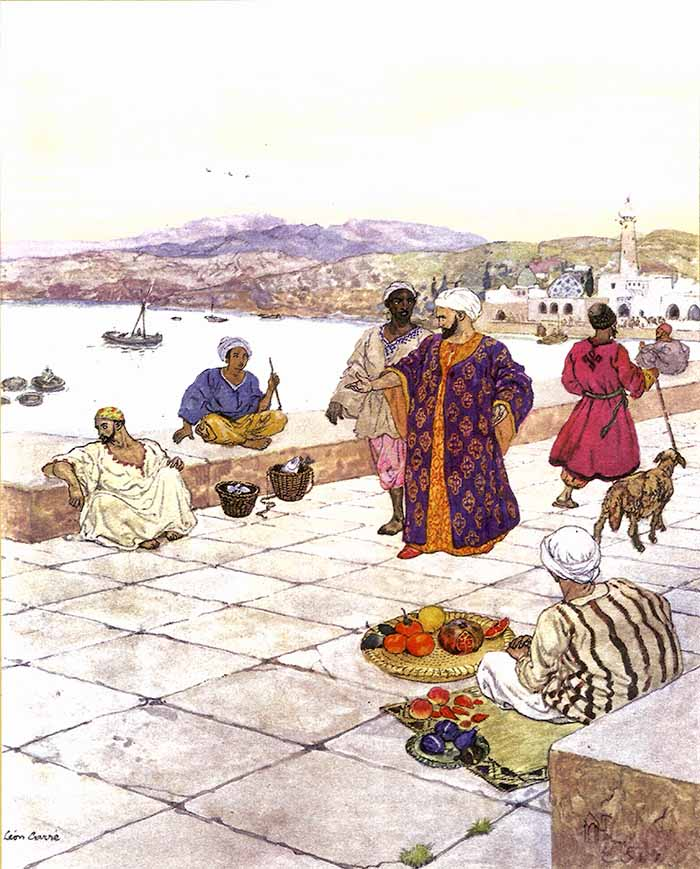
\includegraphics[height=\figsize]{illustrations/volume_5/T05, n0622 - Histoire du dormeur éveillé.jpg}
\end{figure}

\textit{\\
"Tous les soirs il avait coutume d’aller se poster au bout du pont de Bagdad, et là il attendait qu’un étranger vînt à passer ; et dès qu’il en apercevait un, fût-il riche ou pauvre, jeune ou vieux, il s’avançait vers lui, souriant, et plein d’urbanité..."} \\
—T05, n0622 - Histoire du dormeur éveillé \\~\\
\textit{"It was his custom to post himself every evening at the further end of the city bridge and, when he saw a stranger approach, rich or poor, young or old, to accost him with an urbane smile..."} \\
—V03, n0622 - The tale of the sleeper wakened

\newpage

\section{n0629}
\textbf{\Large{The tale of the sleeper wakened}} \\

\begin{figure}[ht]
\centering
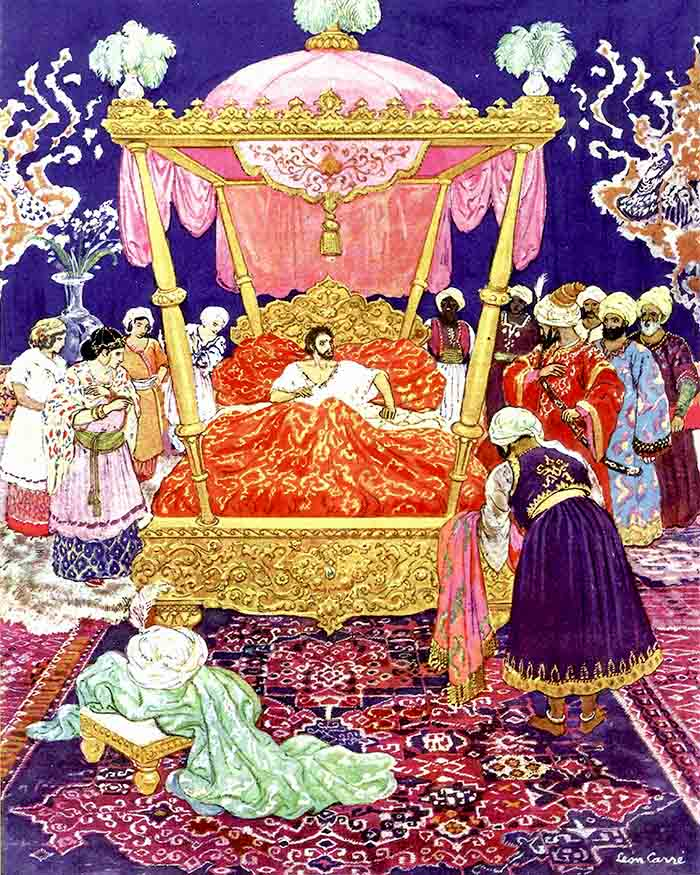
\includegraphics[height=\figsize]{illustrations/volume_5/T05, n0629 - Histoire du dormeur éveillé.jpg}
\end{figure}

\textit{\\
"...Aboul-Hassân finit par sortir de son assoupissement et, s’éveillant, il ouvrit les yeux. Et il se vit d’abord dans un lit magnifique dont la couverture était recouverte d’un brocart d’or rouge constellé de perles et de pierreries !"} \\
—T05, n0629 - Histoire du dormeur éveillé \\~\\
\textit{"Abu al-Hasan came out of his unconsciousness and opened his eyes. He saw a rare bed, covered with a brocade of scarlet gold starred with pearls..."} \\
—V03, n0629 - The tale of the sleeper wakened

\newpage

\section{n0659}
\textbf{\Large{The loves of Zain al-Mawasif}} \\

\begin{figure}[ht]
\centering
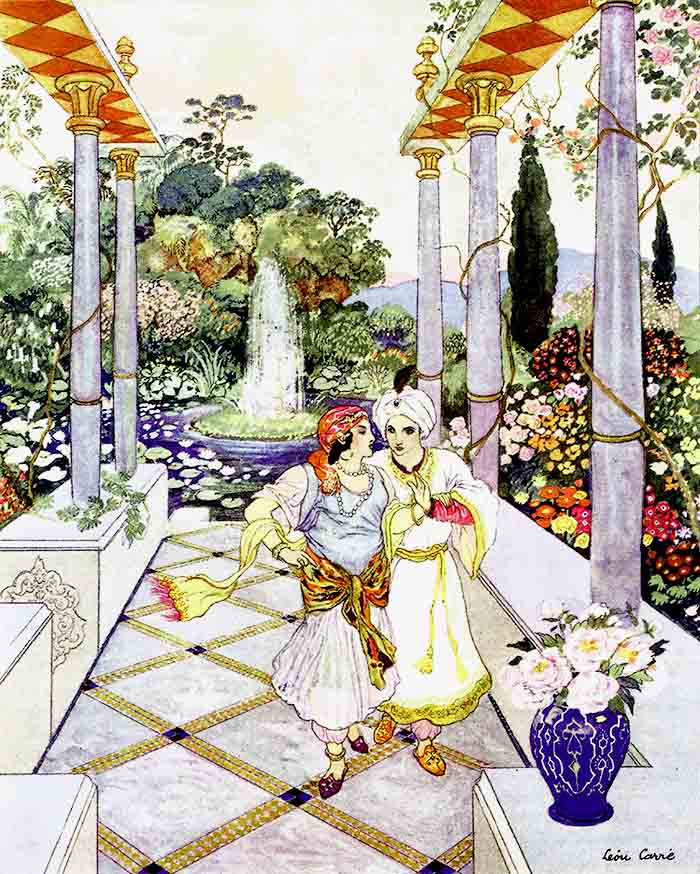
\includegraphics[height=\figsize]{illustrations/volume_5/T05, n0659 - Les amours de Zein Al-Mawassif.jpg}
\end{figure}

\textit{\\
"...ils passèrent la journée l’un près de l’autre, tantôt se reposant et tantôt mangeant et buvant et s’amusant jusqu’au soir."} \\
—T05, n0659 - Les amours de Zein Al-Mawassif \\~\\
\textit{"...the next day they stayed by each other, resting, eating and drinking in joy..."} \\
—V03, n0659 - The loves of Zain al-Mawasif

\newpage

\section{n0663}
\textbf{\Large{The loves of Zain al-Mawasif}} \\

\begin{figure}[ht]
\centering
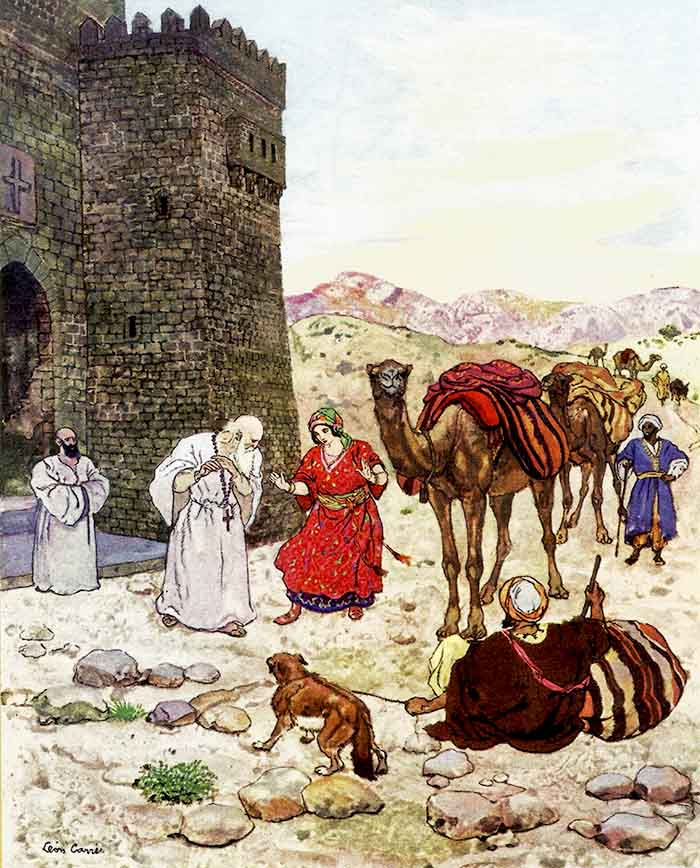
\includegraphics[height=\figsize]{illustrations/volume_5/T05, n0663 - Les amours de Zein Al-Mawassif.jpg}
\end{figure}

\textit{\\
"...le patriarche, à la vue de ce visage de lune, sentit se rajeunir sa vieille chair morte ; et il frémit dans ses pieds, dans son dos, dans son cœur et dans sa tête."} \\
—T05, n0663 - Les amours de Zein Al-Mawassif \\~\\
\textit{"This patriarch, whose name was Danis, sat taking the air outside the door and saw the beautiful girl pass upon her camel; he felt his old dead flesh become alive; his feet shivered, his back shivered, his heart shivered, and his head shivered."} \\
—V03, n0663 - The loves of Zain al-Mawasif

\end{document}